%==============================================================================
\FloatBarrier
%------------------------------------------------------------------------------
\section{Raster plots}
\label{sec:pl_rasters}

To inspect the data, we created rastergrams showing every spike detected from an individual recording contact across every trial in every recording session.
Such data visualisation steps afford an overview of the dataset, and are useful to verify the integrity of the data.
Artifacts, such as those whose removal we described in \autoref{sec:pl_preprocessing}, often appear clearly in rastergrams.
For instance, an artifact which occurs at fixed intervals from the stimulus onset such as the monitor-induced artifact (see \autoref{sec:pl_artifact_elimination}) appears as a narrow vertical line (not shown).
% An artifact which arises over a continuous period of time (such as described in \autoref{sec:pl_movement_artifact} and \autoref{sec:pl_empty_trials}) appears as a horizontal line.
Without normalising the spontaneous activity \autoref{sec:pl_san}, inter-session changes in recording properties would result in large session-to-session changes in overall firing rate.


\begin{figure}[p]
    \centering
    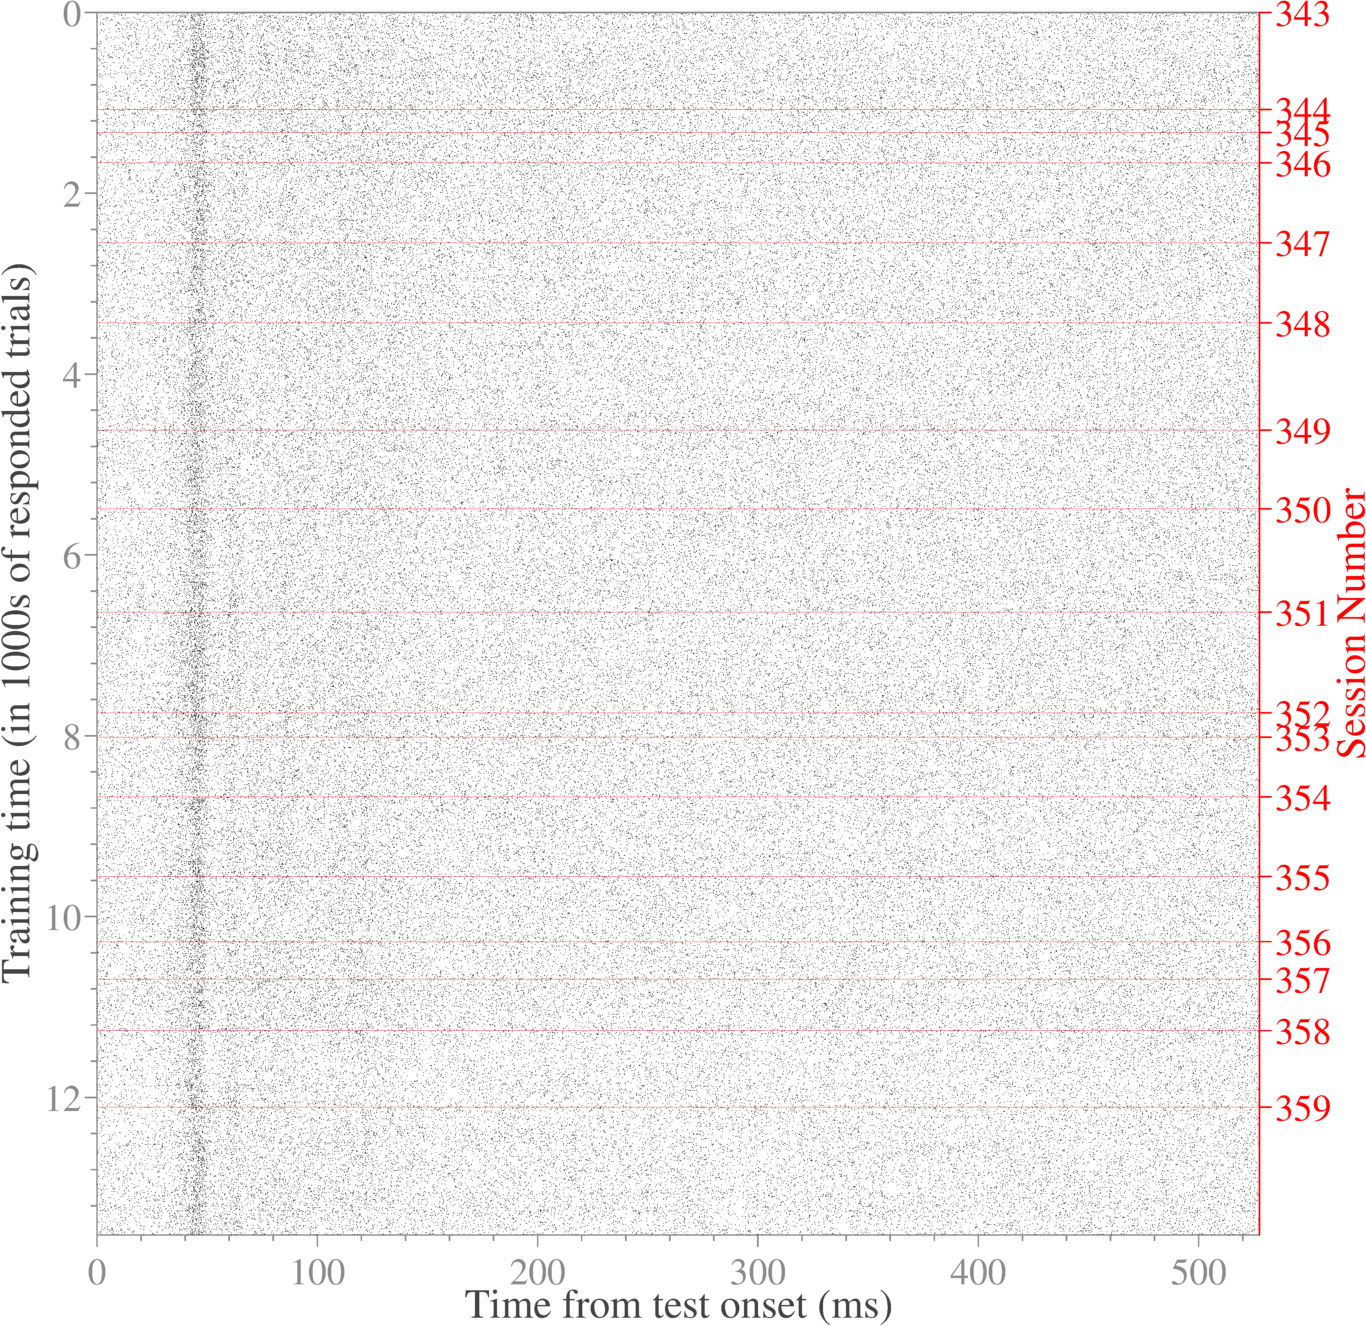
\includegraphics[scale=.35]{%
figs/rasters/rasters_tp4_bw_from-0_to-min_rmvmonitor=2_blanco_v1_1_oc0_ch11_s343-359_.png}
    \caption{\captionemph{Rastergram showing every spike recorded from channel \num{11} of \ac{M1} in \ac{V1} during test stimulus presentation.}
    Along the $x$-dimension, the time since stimulus onset at which the spike was recorded.
    Along the $y$-dimension, the total number of unaborted trials.
    Trials from all experimental sessions are concatenated along the $y$-dimension, with the inter-session breaks indicated by red lines.
}
    \label{fig:raster_blanco_v1}
\end{figure}


\begin{figure}[p]
    \centering
    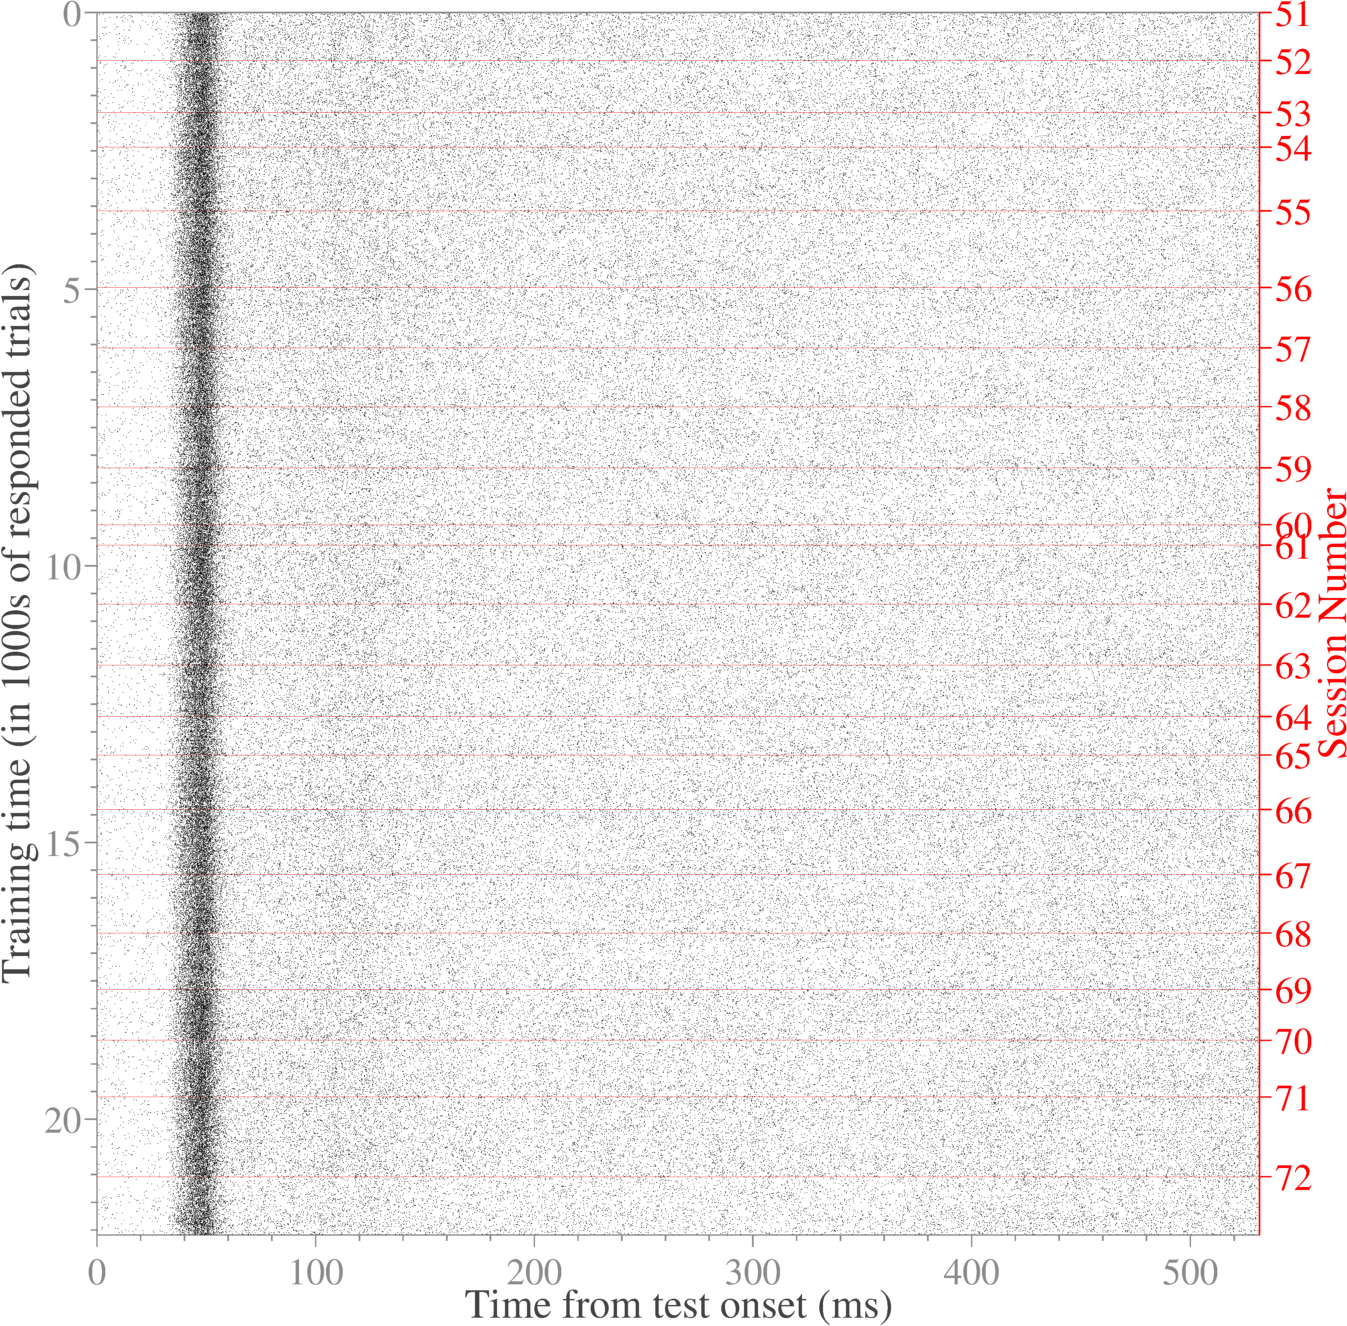
\includegraphics[scale=.35]{%
figs/rasters/rasters_tp4_bw_from-0_to-min_rmvmonitor=2_jack_v1_1_oc0_ch12_s51-72_.png}
    \caption{\captionemph{Rastergram showing every spike recorded from channel \num{12} of \ac{M2} in \ac{V1} during test stimulus presentation.}
    Along the $x$-dimension, the time since stimulus onset at which the spike was recorded.
    Along the $y$-dimension, the total number of unaborted trials.
    Trials from all experimental sessions are concatenated along the $y$-dimension, with the inter-session breaks indicated by red lines.
}
    \label{fig:raster_jack_v1}
\end{figure}


\begin{figure}[p]
    \centering
    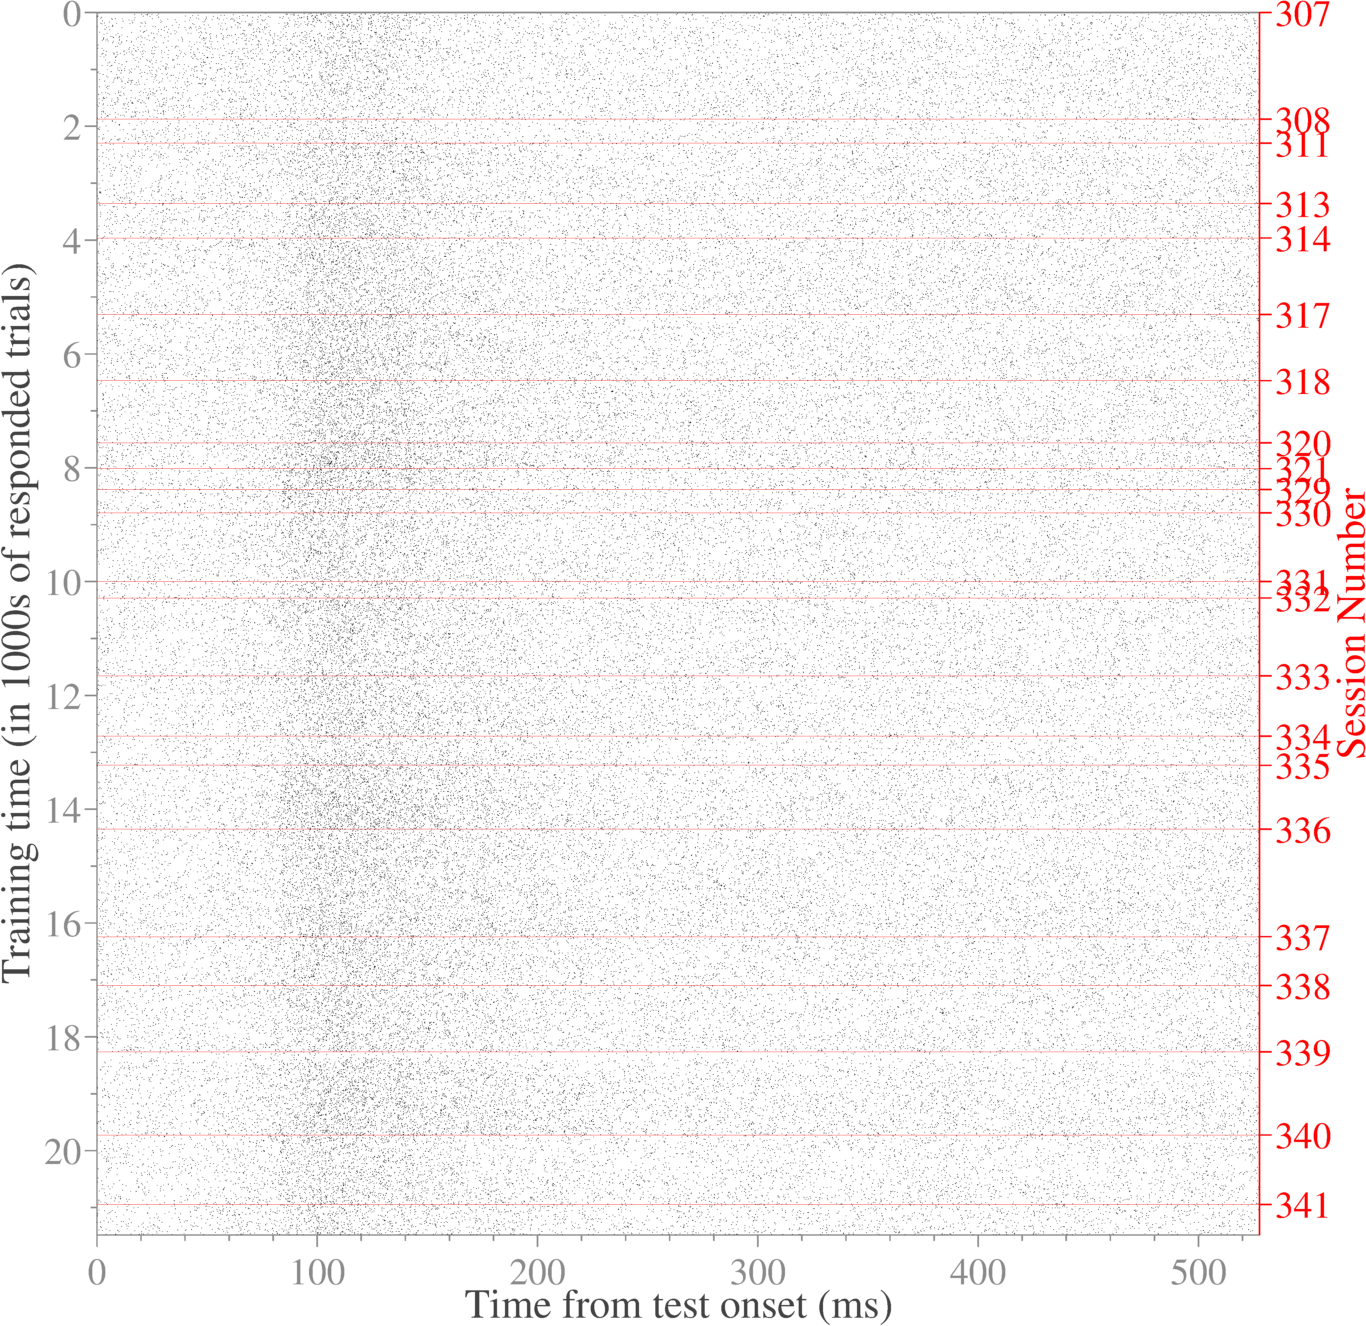
\includegraphics[scale=.35]{%
figs/rasters/rasters_tp4_bw_from-0_to-min_rmvmonitor=2_blanco_v4_1_oc0_ch51_s307,308,311,313,314,317,318,320,321,329-341_.png}
    \caption{\captionemph{Rastergram showing every spike recorded from channel \num{51} of \ac{M1} in \ac{V4} during test stimulus presentation.}
    Along the $x$-dimension, the time since stimulus onset at which the spike was recorded.
    Along the $y$-dimension, the total number of unaborted trials.
    Trials from all experimental sessions are concatenated along the $y$-dimension, with the inter-session breaks indicated by red lines.
}
    \label{fig:raster_blanco_v4}
\end{figure}


\begin{figure}[p]
    \centering
    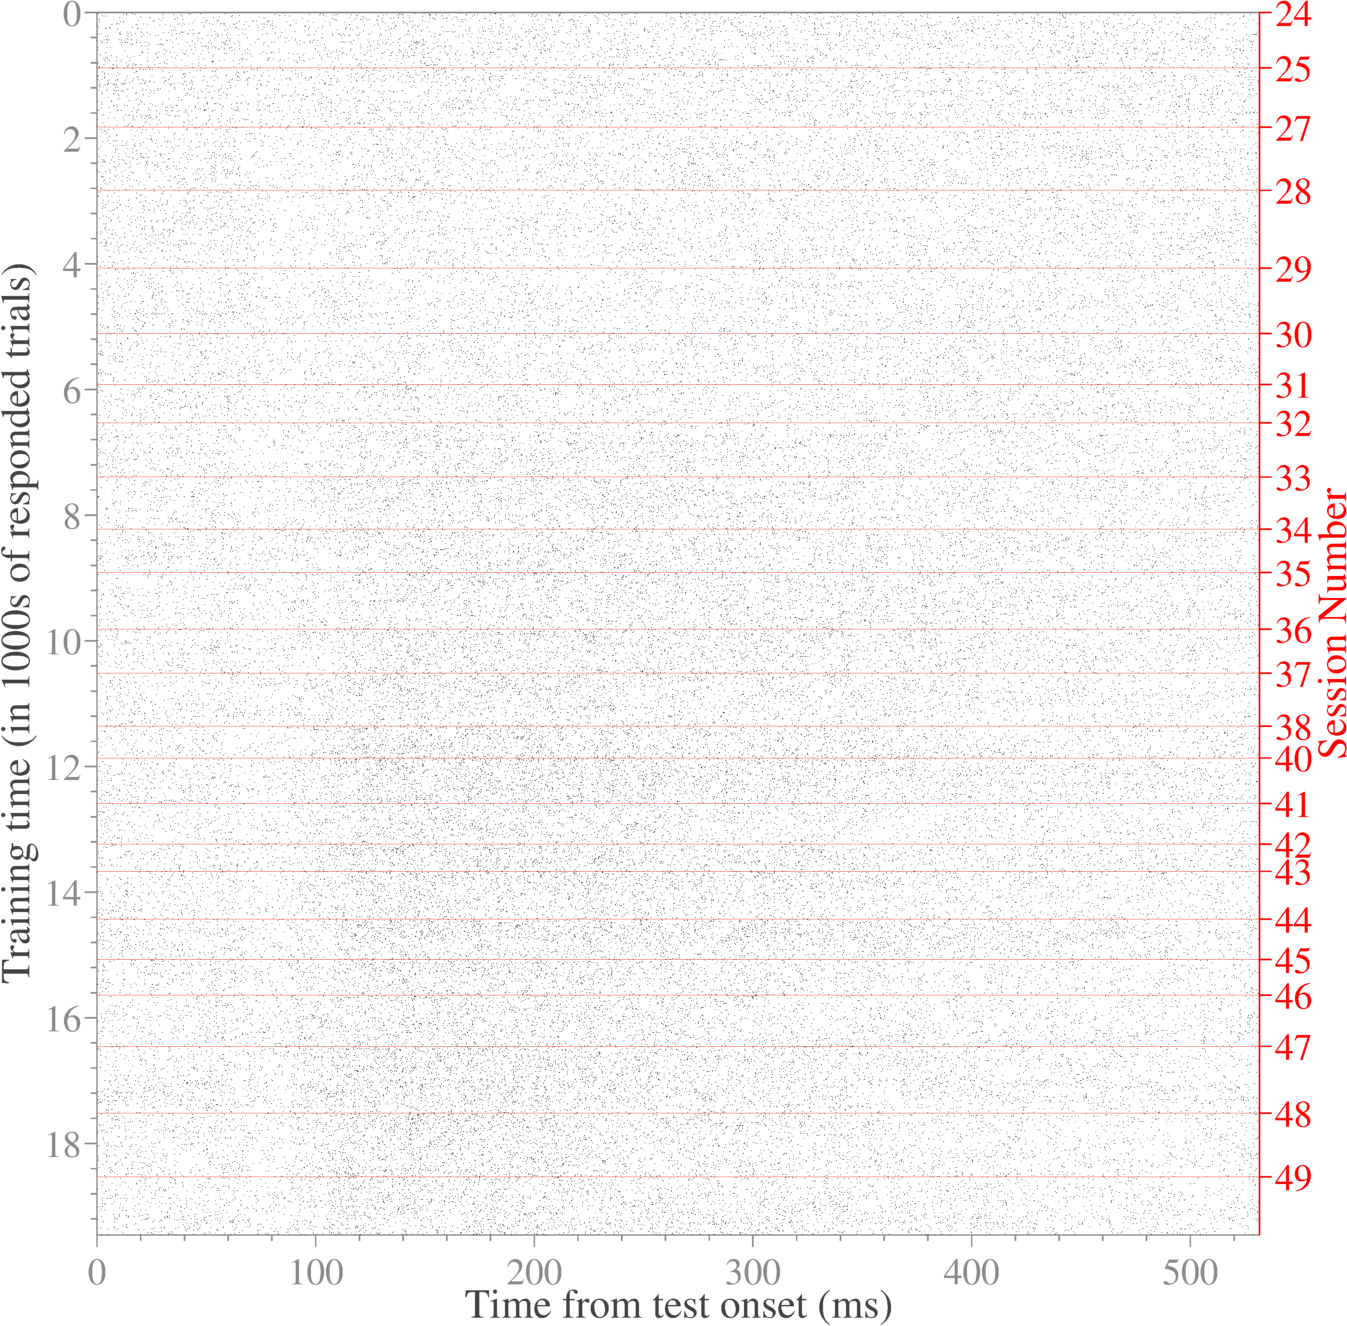
\includegraphics[scale=.35]{%
figs/rasters/rasters_tp4_bw_from-0_to-min_rmvmonitor=2_jack_v4_1_oc0_ch6_s24,25,27-38,40-49_.png}
    \caption{\captionemph{Rastergram showing every spike recorded from channel \num{6} of \ac{M2} in \ac{V4} during test stimulus presentation.}
    Along the $x$-dimension, the time since stimulus onset at which the spike was recorded.
    Along the $y$-dimension, the total number of unaborted trials.
    Trials from all experimental sessions are concatenated along the $y$-dimension, with the inter-session breaks indicated by red lines.
}
    \label{fig:raster_jack_v4}
\end{figure}


In order to familiarise the reader with the data, exemplar rastergrams are shown in Figures \ref{fig:raster_blanco_v1}, \ref{fig:raster_jack_v1}, \ref{fig:raster_blanco_v4}, and \ref{fig:raster_jack_v4}.
We can see that in \ac{V1} (see \autoref{fig:raster_blanco_v1} and \autoref{fig:raster_jack_v1}), there is a peak in the firing rate in response to the stimulus onset, with a delay of approximately \SI{50}{\milli\second}.
Shortly after the stimulus onset response, the neural activity reduces down to a level which is sustained throughout the rest of the stimulus presentation period.
With \ac{M1}, the sustained firing rate is similar to the background rate (a sample of which is shown before the onset response), whereas for \ac{M2} the sustained rate is more clearly elevated versus the background rate.
Although only a single channel is shown for each subject, these properties were common to most of the simultaneously captured neural recordings.
For \ac{V4}, we observe a longer response latency of around \SI{100}{\milli\second} (\autoref{fig:raster_blanco_v4} and \autoref{fig:raster_jack_v4}).
For \ac{M2}, spiking appears to be inhibited before the elevated response begins.

We quantified the change in firing rate evoked by the stimulus relative to the background spontaneous activity with a sensitivity analysis, discussed in \autoref{sec:pl_dprime}.
Next, we will consider the how the firing rate is typically related to the contrast of the stimulus in \autoref{sec:pl_response_curves}.


%------------------------------------------------------------------------------
\section{Stimulus response curves}
\label{sec:pl_response_curves}
%------------------------------------------------------------------------------

By comparing the contrast of the stimulus with the averaged evoked firing rate, we can investigate the relationship between stimulus and response.
For some channels, the multi-unit response recorded was untuned, with the same firing rate evoked by each stimulus, on average (not shown).
For most channels, there was a stimulus dependent response which increased monotonically .
Some channels showed a more highly tuned response than others, indicated by a steeper response curve or reduced noise (measured as the standard deviation of the response over repetitions).
Example contrast tuning curves, which are stereotypical for the tuned responses we observed, are shown in \autoref{fig:respcurve}.


\begin{figure}[htbp]
    \centering
    \hspace*{\fill}
    \subfloat[\ac{M1} \ac{V1}, channel \num{11}, session \num{359}.\label{fig:respcurve_v1_blanco}]{
        \centering
        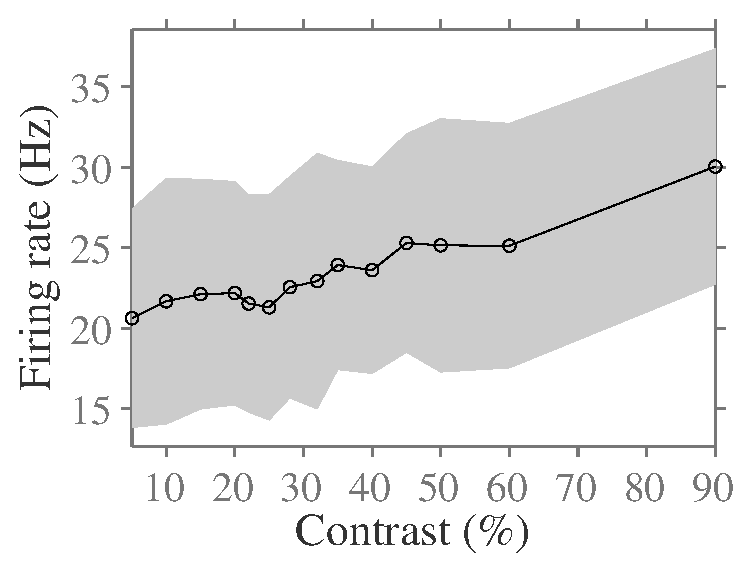
\includegraphics[scale=.45]{%
figs/response_curve/respcurve_blanco_v1_ch11_s359.eps}
    }
    \hspace{.4cm}
    \subfloat[\ac{M2} \ac{V1}, channel \num{12}, session \num{72}.\label{fig:respcurve_v1_jack}]{
        \centering
        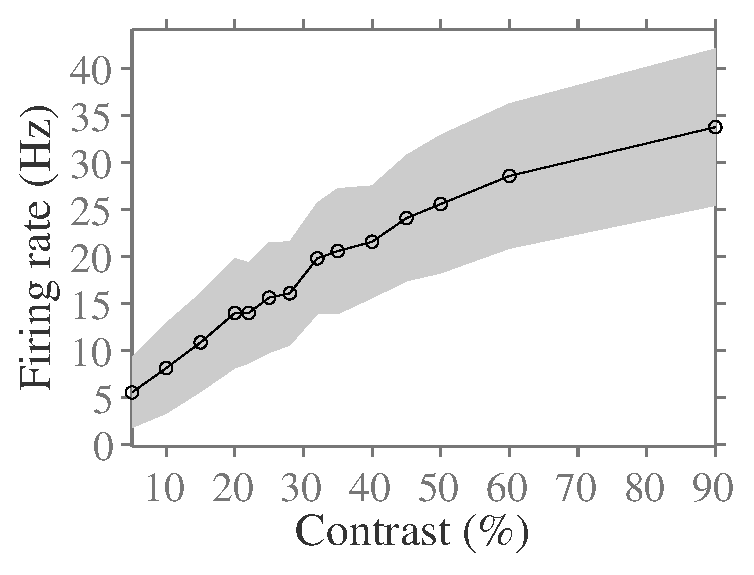
\includegraphics[scale=.45]{%
figs/response_curve/respcurve_jack_v1_ch12_s72.eps}
    }
    \hspace*{\fill}
    \\
    \hspace*{\fill}
    \subfloat[\ac{M1} \ac{V4}, channel \num{51}, session \num{341}.\label{fig:respcurve_v4_blanco}]{
        \centering
        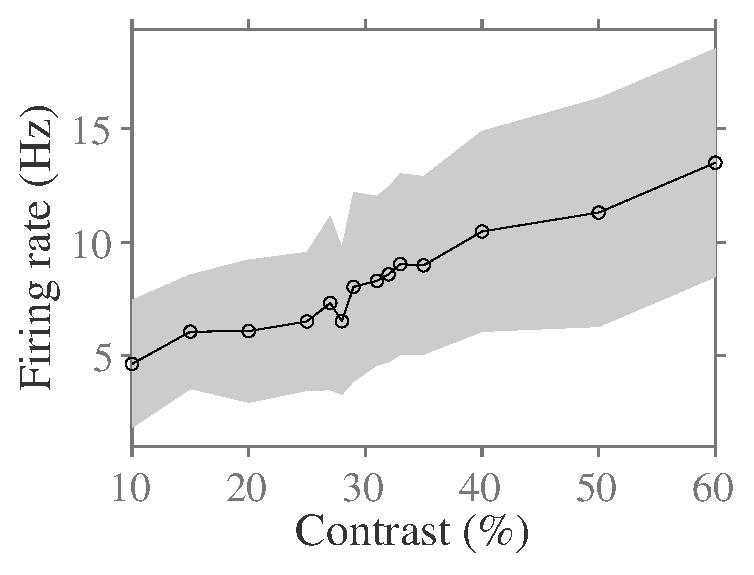
\includegraphics[scale=.45]{%
figs/response_curve/respcurve_blanco_v4_ch51_s341.eps}
    }
    \hspace{.4cm}
    \subfloat[\ac{M2} \ac{V4}, channel \num{6}, session \num{49}.\label{fig:respcurve_v4_jack}]{
        \centering
        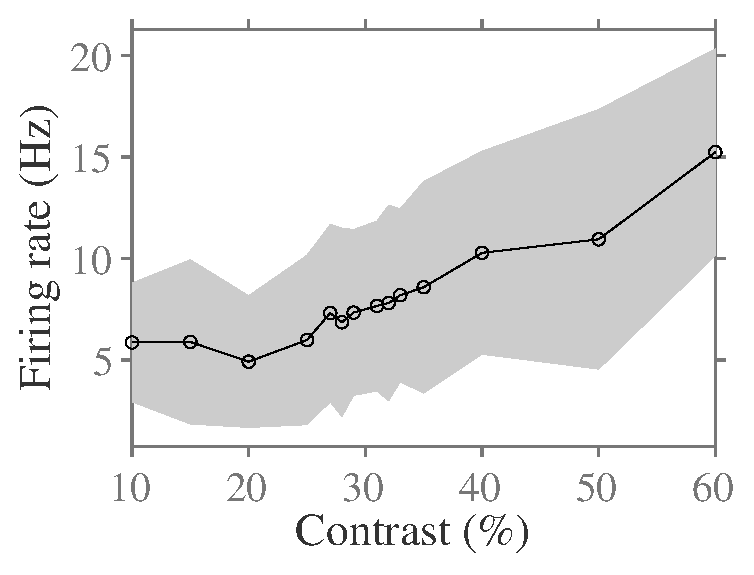
\includegraphics[scale=.45]{%
figs/response_curve/respcurve_jack_v4_ch6_s49.eps}
    }
    \hspace*{\fill}
    \caption{\captionemph{Stimulus response tuning curves.}
    In each subfigure, we show the firing rate evoked by each test stimulus during the final recording session.
    The average firing rate is shown (black line), along with the standard deviation over all stimulus repetitions (shaded grey region).
}
    \label{fig:respcurve}
\end{figure}
